
%!TEX ROOT=ctutest.tex

\chapter{Identifikované parametry}
\label{identifikovane_parametry_ch}
Postupem popsaným v sekci \ref{postup_identifikace_ch} byly identifikovány všechny neznámé parametry. Identifikované parametry jsou uvedeny v tabulce \ref{tab_ind_hodnot}. V následující tabulce \ref{tab_ind_hodnot_3d} jsou pro srovnání vypsané hodnoty identifikované z 3D modelu robotu (viz sekce \ref{z_3d_modelu_sec}). Hodnoty hmotností, momentů setrvačnosti a poloh těžiště v tabulkách jsou uvedeny v základních jednotkách SI. Koeficienty tření jsou bezrozměrné.
\\
\begin{table}[htbp]
  \centering
  \caption{Tabulka parametrů identifikovaných z rovnic}
    \begin{tabular}{c|cccccccccc}
    \multicolumn{1}{c|}{Osa} & \multicolumn{1}{c}{$I_{xx}$} & \multicolumn{1}{c}{$I_{yy}$} & \multicolumn{1}{c}{$I_{zz}$} & \multicolumn{1}{c}{$d_x$} & \multicolumn{1}{c}{$d_y$} & \multicolumn{1}{c}{$d_z$} & \multicolumn{1}{c}{$m$} & \multicolumn{1}{c}{$f_v$} & \multicolumn{1}{c}{$f_c$} \\
    \hline
    1  & 0     & 0     & 3.963 & 0     & 0     & 0     & 0     & 93.540 &  6.473 \\
    2  & 0.197 & 3.078 & 1.967 & 0.301 & 0.034 & 0     & 19.30 & 93.240 & 21.107 \\
    3  & 0.490 & 3.025 & 0.799 &-0.038 &-0.133 &-0.006 & 26.47 & 24.510 &  2.486 \\
    4  & 1.737 & 0.509 & 0.637 &-0.037 & 0.024 &-0.027 & 7.41  &  7.235 &  1.594 \\
    5  & 0.105 & 0.353 & 0.218 & 0.030 & 0     &-0.140 & 2.53  &  1.863 &  1.033 \\
    6  & 0.179 & 0.206 & 0.027 & 0     & 0     & 0.133 & 0.60  &  1.148 &  0.396 \\
    \end{tabular}%
  \label{tab_ind_hodnot}%
\end{table}%

\begin{table}[htbp]
  \centering
  \caption{Tabulka parametrů identifikovaných z 3D modelu}
    \begin{tabular}{c|cccccccccc}
    \multicolumn{1}{c|}{Osa} & \multicolumn{1}{c}{$I_{xx}$} & \multicolumn{1}{c}{$I_{yy}$} & \multicolumn{1}{c}{$I_{zz}$} & \multicolumn{1}{c}{$d_x$} & \multicolumn{1}{c}{$d_y$} & \multicolumn{1}{c}{$d_z$} & \multicolumn{1}{c}{$m$} \\
    \hline
    1  & 0.322   & 0.467   & 0.478   & 0.091 & 0.067 & 0.006 & 26.98 \\
    2  & 0.541   & 0.552   & 0.044   & 0.333 & 0.002 & 0.039 & 15.92 \\
    3  & 0.775   & 0.750   & 0.210   &-0.032 &-0.008 &-0.034 & 25.85 \\
    4  & 0.010   & 0.020   & 0.024   & 0     & 0.109 &-0.008 & 4.09  \\
    5  & 0.002   & 0.004   & 0.004   & 0     &-0.01  & 0     & 1.62  \\
    6  & 0.00006 & 0.00003 & 0.00003 & 0     & 0     & 0.111 & 0.02  \\
    \end{tabular}%
  \label{tab_ind_hodnot_3d}%
\end{table}%

Porovnáním hodnot v obou tabulkách je patrné, že se většina parametrů, s výjimkou hmotností ramen, poměrně výrazně liší. Dalším rozdílem je, že z 3D modelu není možné získat informace o koeficientech tření v jednotlivých osách, zatímco identifikace z rovnic se třením počítá. Vliv tření na přesnost modelu je analyzován v další části.

\section{Simulace odvozených parametrů}

Na následujících obrázcích (obr. \ref{osa_1_sim_pic} až \ref{osa_6_sim_pic}) jsou odsimulované průběhy točivých momentů s odvozenými parametry všech šesti os. Jsou v nich odsimulované predikované průběhy točivých momentů modelem s parametry odvozenými pomocí rovnic a pomocí 3D modelu. 

Simulace je provedena tak, že byl nejprve s robotem vykonán pohyb po určité trajektorii. Přitom byly měřeny průběhy poloh, úhlových rychlostí, úhlových zrychlení a momentů sil. Polohy, rychlosti a zrychlení byly následně dosazeny do odvozených identifikovaných modelů a výsledné momenty sil byly porovnány se změřenými.

Protože z 3D modelu není možné získat koeficienty tření os, je zde možnost uvažovat tyto koeficienty jako nulové a tím je v modelu zanedbat. Tento model je ale velmi nepřesný (viz průběhy \ref{osy_sim_pic}). Na průbězích je vidět, že vychází opravdu velmi vysoké odchylky od naměřených dat. Tření os hraje v dynamice robota významnou roli, proto ho není možné tímto způsobem zanedbat.

Odvozené parametry z 3D modelu je možné využít tak, že se budou v dynamických rovnicích uvažovat jako známé a z rovnic se odvodí pouze neznámé koeficienty tření. Na průbězích níže jsou pro srovnání odsimulované průběhy s parametry získanými tímto způsobem. 

\begin{figure}[h]
    \centering
    \begin{subfigure}[b]{1\textwidth}
        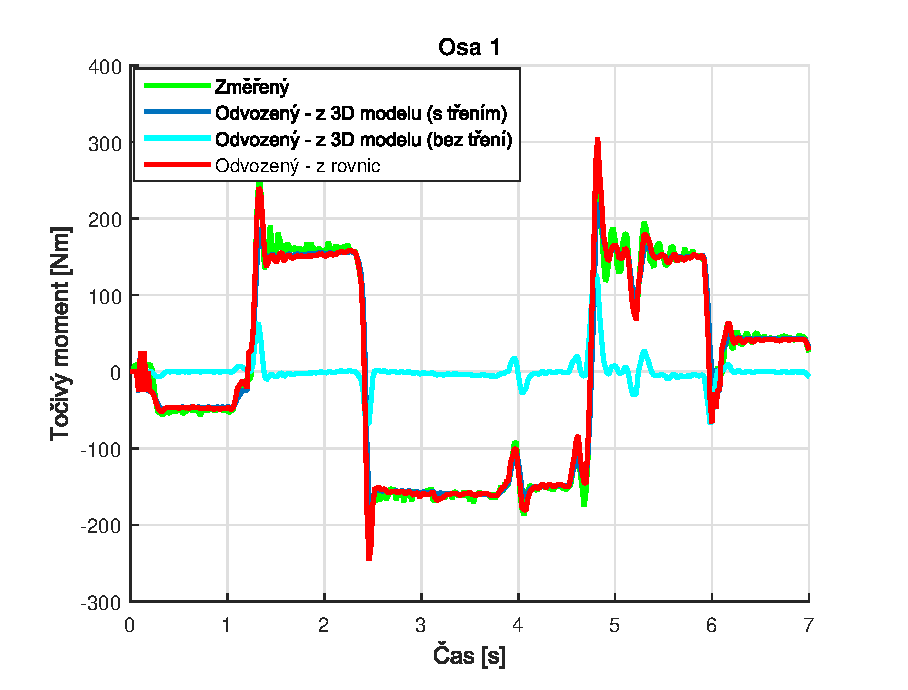
\includegraphics[width=\textwidth]{Osa_1_sim}
        \caption{Osa 1}
        \label{osa_1_sim_pic}
        \end{subfigure}
\end{figure}
\begin{figure}\ContinuedFloat    
    \begin{subfigure}[b]{1\textwidth}
        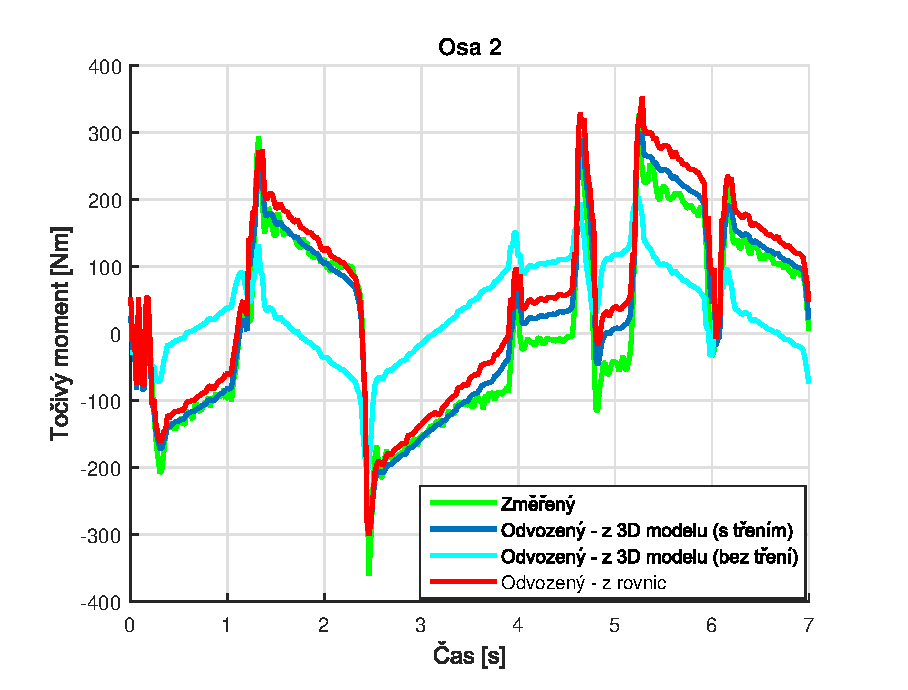
\includegraphics[width=\textwidth]{Osa_2_sim}
        \caption{Osa 2}
        \label{osa_2_sim_pic}
    \end{subfigure}
    \begin{subfigure}[b]{1\textwidth}
        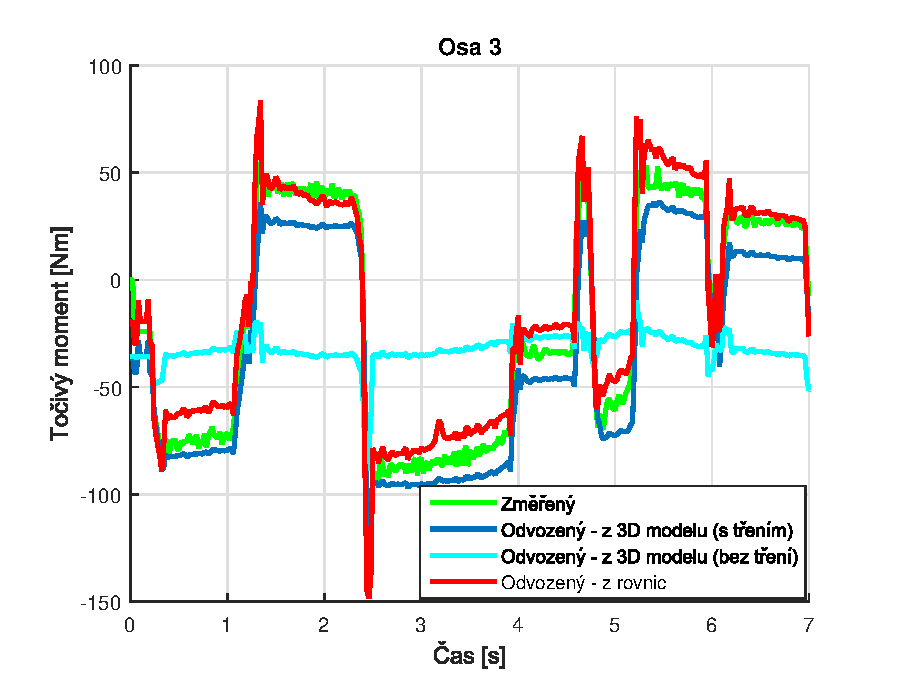
\includegraphics[width=\textwidth]{Osa_3_sim}
        \caption{Osa 3}
        \label{osa_3_sim_pic}
    \end{subfigure}
\end{figure}
\begin{figure}\ContinuedFloat
    \begin{subfigure}[b]{1\textwidth}
        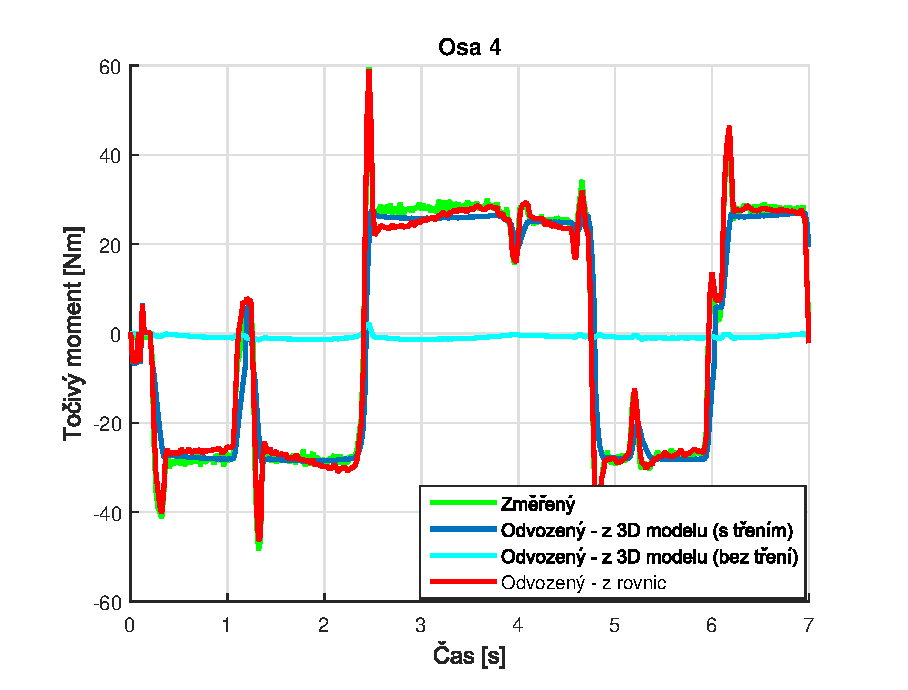
\includegraphics[width=\textwidth]{Osa_4_sim}
        \caption{Osa 4}
        \label{osa_4_sim_pic}
    \end{subfigure}
    \begin{subfigure}[b]{1\textwidth}
        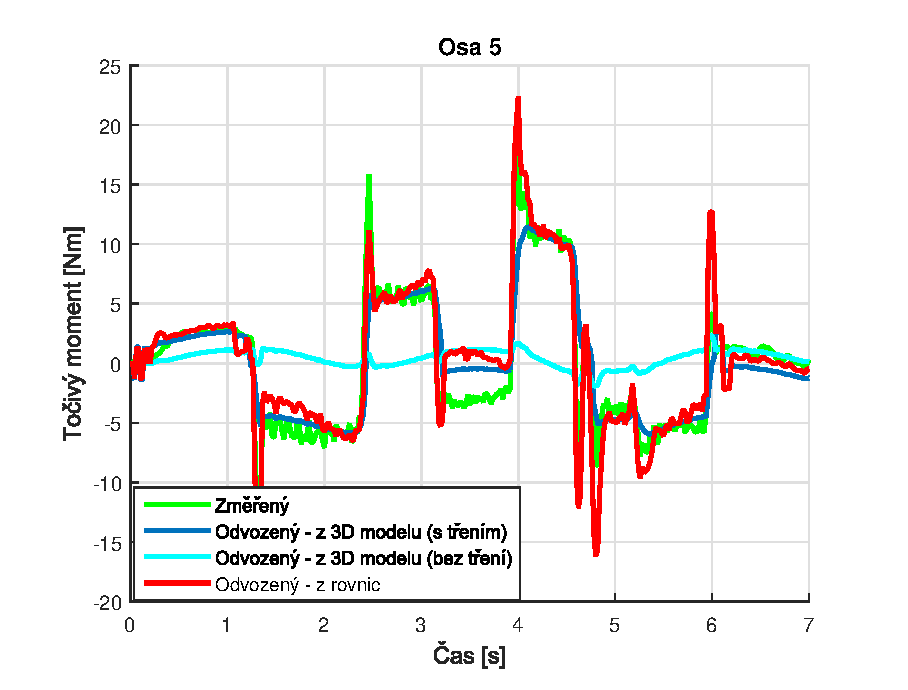
\includegraphics[width=\textwidth]{Osa_5_sim}
        \caption{Osa 5}
        \label{osa_5_sim_pic}
    \end{subfigure}
\end{figure}

\clearpage

\begin{figure}\ContinuedFloat
    \begin{subfigure}[b]{1\textwidth}
        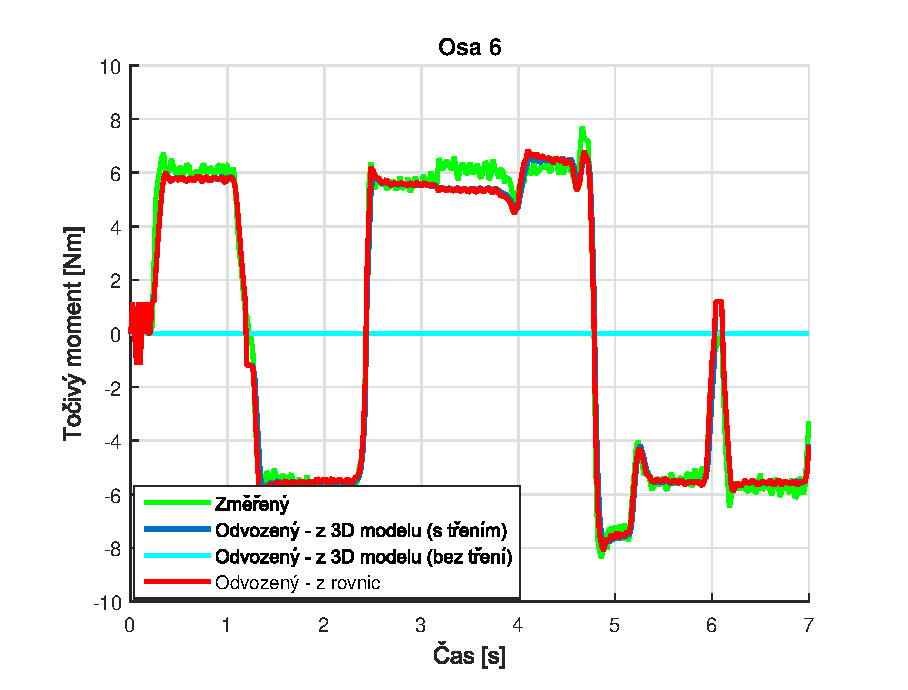
\includegraphics[width=\textwidth]{Osa_6_sim}
        \caption{Osa 6}
        \label{osa_6_sim_pic}
    \end{subfigure}
    \caption{Srovnání měření se simulacemi s odvozenými parametry}\label{osy_sim_pic}
\end{figure}

Z výše uvedených průběhů je patrné, že v případě zanedbání tření os je získaný model robotu nepoužitelný. Nejlepších výsledků tento model dosahuje na ose 2 kde mají na dynamiku kromě tření velký vliv také hmotnosti a polohy těžišť následujících ramen, jejichž hmotnost osa 2 nese. Naopak například pro osy 4 a 6 je vliv ostatních parametrů vůči tření na této trajektorii zanedbatelný, proto jsou predikované momenty na těchto osách téměř nulové. Z toho důvodu se nadále již model se zanedbaným třením neuvažuje.

Naopak model s identifikovanými parametry pomocí analytických rovnic a pomocí 3D modelu se třením poskytuje poměrně přesné předpovědi. Ve většině případů jsou predikované hodnoty z modelu téměř totožné s těmi změřenými. Na následujících obrázcích (\ref{osa_1_odch_pic} až \ref{osa_6_odch_pic}) je srovnání odchylek obou modelů. V grafech je znázorněna okamžitá a průměrná absolutní odchylka mezi modely a měřením.

\begin{figure}[h]
    \centering
    \begin{subfigure}[b]{0.7\textwidth}
        \includegraphics[width=\textwidth]{Osa_1_odch}
        \caption{Osa 1}
        \label{osa_1_odch_pic}
    \end{subfigure}
    \begin{subfigure}[b]{0.7\textwidth}
        \includegraphics[width=\textwidth]{Osa_2_odch}
        \caption{Osa 2}
        \label{osa_2_odch_pic}
    \end{subfigure}
    \begin{subfigure}[b]{0.7\textwidth}
        \includegraphics[width=\textwidth]{Osa_3_odch}
        \caption{Osa 3}
        \label{osa_3_odch_pic}
    \end{subfigure}
\end{figure}
\begin{figure}\ContinuedFloat
    \begin{subfigure}[b]{0.7\textwidth}
        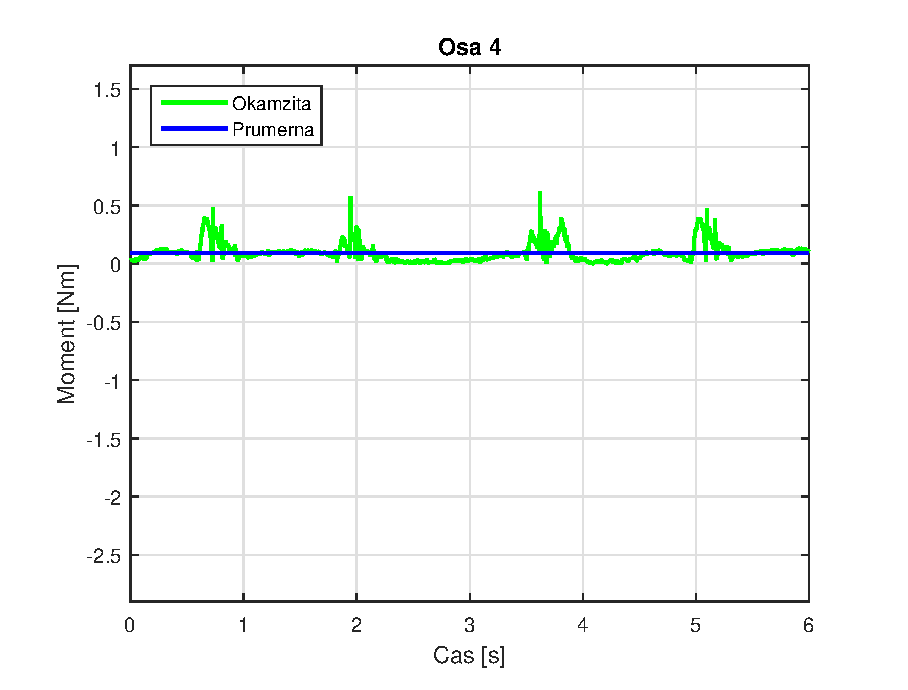
\includegraphics[width=\textwidth]{Osa_4_odch}
        \caption{Osa 4}
        \label{osa_4_odch_pic}
    \end{subfigure}
    \begin{subfigure}[b]{0.7\textwidth}
        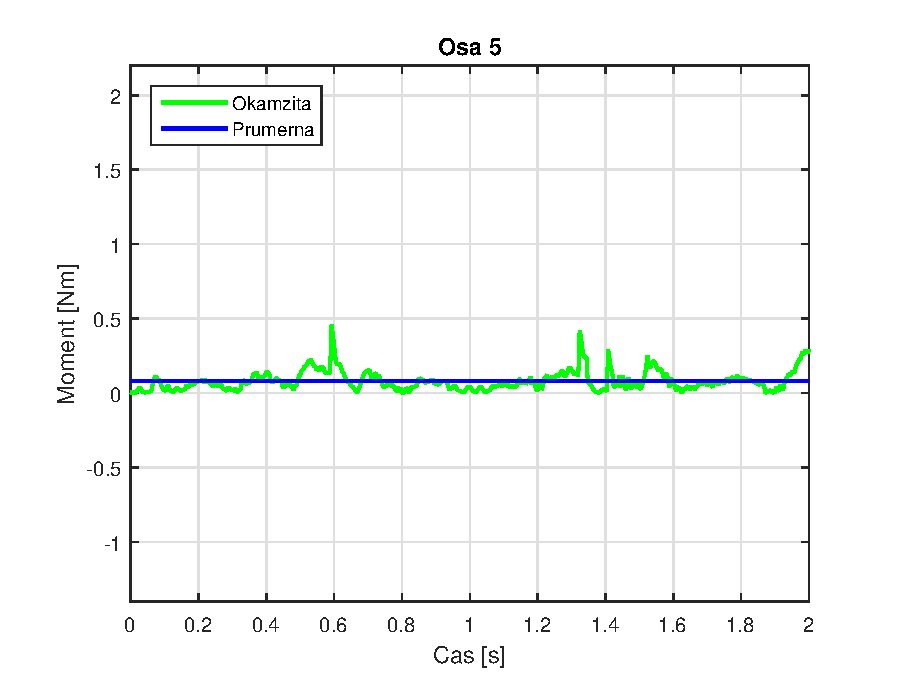
\includegraphics[width=\textwidth]{Osa_5_odch}
        \caption{Osa 5}
        \label{osa_5_odch_pic}
    \end{subfigure}
    \begin{subfigure}[b]{0.7\textwidth}
        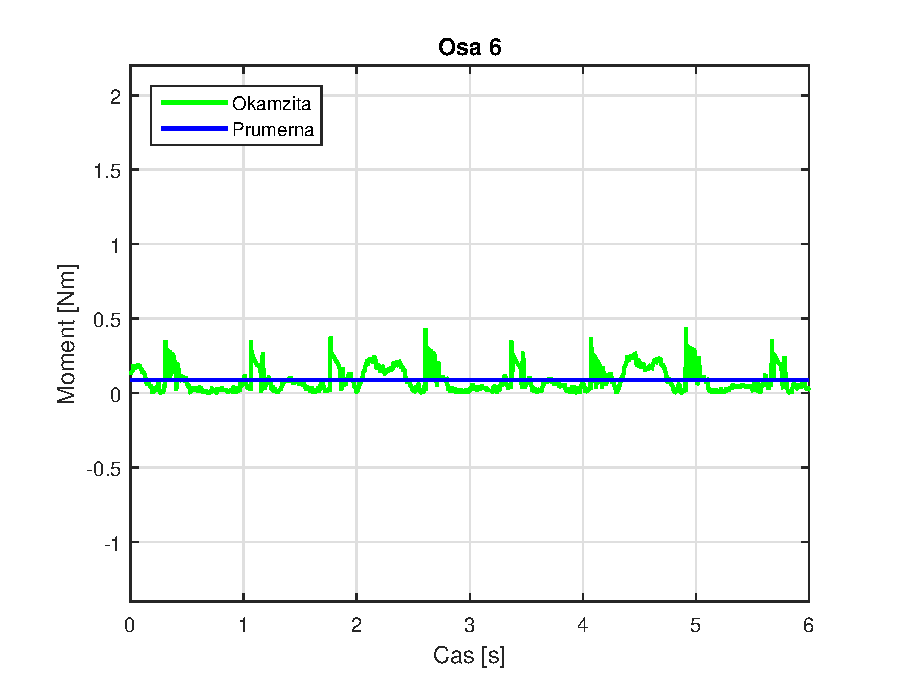
\includegraphics[width=\textwidth]{Osa_6_odch}
        \caption{Osa 6}
        \label{osa_6_odch_pic}
    \end{subfigure}
    \caption{Srovnání odchylek modelů a měření}\label{osy_odch_pic}
\end{figure}

\clearpage

Z grafů je patrné, že oba modely jsou podobně přesné. Na osách 1, 5 a 6 se průměrné odchylky obou metod překrývají. Z průběhů je možné také vypozorovat, že model identifikovaný z rovnic dokáže lépe modelovat ostré špičky na momentech. Pro přesnější srovnání jsou v tabulce \ref{tab_srov_odch} uvedeny přesné hodnoty průměrných odchylek na jednotlivých osách.

\hfill
\begin{table}[htbp]
  \centering
  \caption{Srovnání středních odchylek modelů vůči měření}
    \begin{tabular}{c|cc|cc}
          & \multicolumn{2}{c|}{Analytické rovnice} & \multicolumn{2}{c}{3D model [Nm]} \\
    Osa   & Absolutní [Nm] & Relativní [\%]  & Absolutní [Nm] & Relativní [\%] \\
    \hline
    1     & 9,99  & 8,10  & 11,86 & 9,57  \\
    2     & 43,77 & 30,30 & 24,20 & 15,52 \\
    3     & 9,33  & 17,48 & 13,20 & 24,73 \\
    4     & 1,91  & 7,01  & 4,94  & 18,13 \\
    5     & 1,60  & 25,84 & 1,69  & 28,33 \\
    6     & 0,46  & 8,07  & 0,52  & 9,12  \\
    \end{tabular}%
  \label{tab_srov_odch}%
\end{table}%

Porovnáním odchylek těchto dvou metod identifikace v tabulce \ref{tab_srov_odch} je možné říct, že obě metody dávají srovnatelné modely. Podle předpokladů má metoda identifikace z rovnic nižší odchylky od změřených hodnot na většině os. Výjimkou je osa 2. Odchylky na osách 5 a 6 jsou prakticky stejné pro obě metody. Největší nepřesnost je na ose 2, kde model identifikovaný z 3D modelu dosahuje lepších výsledků. Důvodem větší nepřesnosti metody z rovnic může být nedostatečně excitující identifikační trajektorie pro osu 2.

Identifikace z rovnic pomocí excitační trajektorie tedy obecně dává přesnější model robota. Navíc k tomu aby metoda identifikace z 3D modelu dávala rozumně přesný model, je k němu nutné pomocí rovnic identifikovat koeficienty tření. Proto je dále pro modelování spotřeby robota použit model identifikovaný pomocí rovnic.